% SIAM Article Template
% remove review to surprass the wtermark at the end of every page
%\documentclass[review,hidelinks,onefignum,onetabnum]{siamart220329}

\documentclass[hidelinks,onefignum,onetabnum]{siamart220329}
% Information that is shared between the article and the supplement
% (title and author information, macros, packages, etc.) goes into
% ex_shared.tex. If there is no supplement, this file can be included
% directly.

% SIAM Shared Information Template
% This is information that is shared between the main document and any
% supplement. If no supplement is required, then this information can
% be included directly in the main document.


% Packages and macros go here

\usepackage{amsfonts}
\usepackage{graphicx}
\usepackage{epstopdf}
\usepackage{multirow}
\usepackage{hyperref}
\usepackage{algorithmic}
\ifpdf
  \DeclareGraphicsExtensions{.eps,.pdf,.png,.jpg}
\else
  \DeclareGraphicsExtensions{.eps}
\fi

% Add a serial/Oxford comma by default.
\newcommand{\creflastconjunction}{, and~}

% Used for creating new theorem and remark environments
\newsiamremark{remark}{Remark}
\newsiamremark{hypothesis}{Hypothesis}
\crefname{hypothesis}{Hypothesis}{Hypotheses}
\newsiamthm{claim}{Claim}

% Sets running headers as well as PDF title and authors
\headers{Explaining NonLinear Classification Decisions}{Marcel Pommer}

% Title. If the supplement option is on, then "Supplementary Material"
% is automatically inserted before the title.
\title{Explaining NonLinear Classification Decisions with Deep Taylor Decompositions
\thanks{Submitted to professor Kutyniok on the 03.07.2022}}

% Authors: full names plus addresses.
\author{Marcel Pommer}

\usepackage{amsopn}
\DeclareMathOperator{\diag}{diag}


%%% Local Variables: 
%%% mode:latex
%%% TeX-master: "ex_article"
%%% End: 


% Optional PDF information
\ifpdf
\hypersetup{
  pdftitle={Explaining NonLinear Classification Ddecisions with Deep Taylor Decompositions an analyysis},
  pdfauthor={Marcel Pommer}
}
\fi

% The next statement enables references to information in the
% supplement. See the xr-hyperref package for details.

%\externaldocument[][nocite]{ex_supplement}

% FundRef data to be entered by SIAM
%<funding-group specific-use="FundRef">
%<award-group>
%<funding-source>
%<named-content content-type="funder-name"> 
%</named-content> 
%<named-content content-type="funder-identifier"> 
%</named-content>
%</funding-source>
%<award-id> </award-id>
%</award-group>
%</funding-group>

\begin{document}

\maketitle

% REQUIRED
\begin{abstract}
During the last decade Deep Neural Networks (DNNs) as well as other sophisticated machine learning models gained substantially on relevance, due to so far unreached performance in a variety of topics like image recognition, classification or natural language processing, to name only a few. Despite their great performance those, mostly non linear models, lack of one important aspect, the explainability of the results. Montavon et al. introduce in their paper \textit{Explaining NonLinear Classification Decisions with Deep Taylor Decompositions} a new technique, the deep taylor decomposition, to map the relevance of the output on the input features, i.e. quantify the influence of each input variable on the output. They demonstrate the results on two image recognition data sets, the MNIST and the ILSVRC, creating heatmaps to display the relevance of the single pixel. I recreate the procedure in Python and apply the deep taylor decomposition to a non image recognition data set, the titanic dataset.
\end{abstract}

% REQUIRED
\begin{keywords}
Explainability, Deep Neural Networks, Image Recognition
\end{keywords}

% REQUIRED
\begin{MSCcodes}
62H35, 93B15
\end{MSCcodes}

\section{Introduction}
The raise of machine learning, combined with steadily growing computational power revolutionized many so far hard to grasp tasks like image recognition in order to push the development of self driving cars, help to diagnose deseases or automate classification problems. One can think of a variety of different models like random forests, boosting or deep neural networks and maybe even of more applications in our daily lives, beginning with the advertisement displayed in our browser, or the netflix recommendations going to automated voice recgonition and translation to comunicate with people all over the world. Those new techniques became quite famous during the last decade due to their overperformance in nearly ever field, however their complexity makes them mathematicaly hard to understand and explain leading to one of their major drawbacks, missing explainability. The paper \textit{Explaining NonLinear Classification Decisions with Deep Taylor Decompositions} [XXX] by Montavon et al. tries to tackle this problem by extending the explainability of deep neural networks using taylor expansion, resulting in a mapping of non negative relevance from the output to each input feature. The authors apply their technique to a variety of exmaples from the MNIST [XXX] dataset as well as the ILSVRC [XXX] dataset. In figure 1 one can see a tractable example, in which a neural network detects a `0` while distracted by a `5`. We denote the neurons with $x_i$ and the respective contributions with $R_i$, resulting in a graphical representation, i.e. a heatmap, indicating which pixels contribut with which intensity to the decision of the neural network.
\begin{figure}[ht]
	\centering
      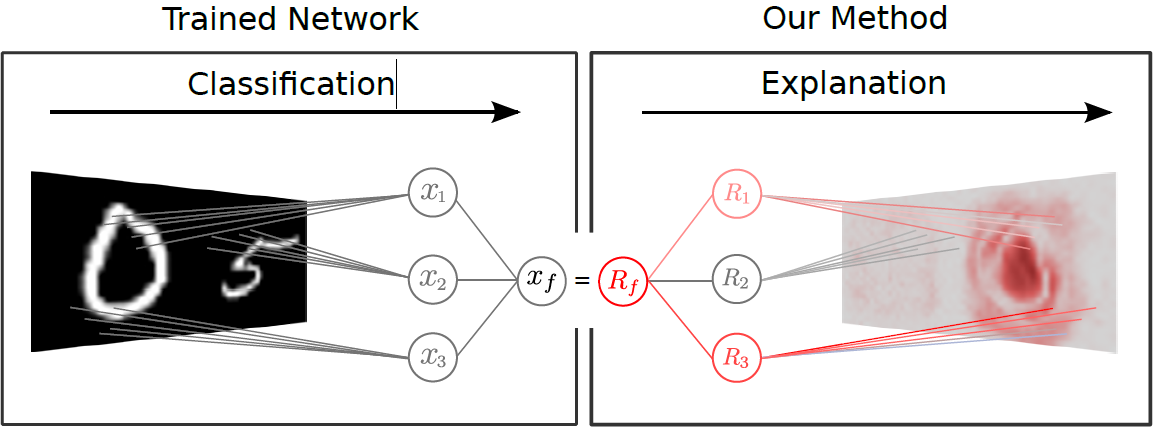
\includegraphics[width=0.5\textwidth]{images/fig._1_example}
	\caption{Example: Detecting 0 while distrecting other numbers are in place with a neural network}
	\label{fig.1}
\end{figure}
Montavon et al. focus on image recognition in their paper, but highlight, that the procedure can be broadcasted to any input space and feature set. In my analysis of the application of the algorithm I will focus on the titanic [XXX] dataset which is very tractable and easy to understand and interpret.

% The outline is not required, but we show an example here.
The paper is organized as follows. The main results are in
\ref{sec:main}, the application on a simple neural network and algorithms in  section \ref{sec:alg}, examples on the MNIST data set and experiments on the titanic dataset in section \ref{sec:exp}, and the conclusion follows in section \ref{sec:conclusions}.

\section{Main results}
\label{sec:main}

In this section I will describe the general idea of the deep taylor decomposition, present the definitions and theorems as well as some handy examples. Since the authors focus on image recognition in their analysis I will follow this methodology, however in section \ref{sec:experiments} I will transfer all results to a simple regression task. In the context of image classification, we define the d-dimensional input $x \in\mathbb{R}^d$, where the image pixels ($p$) can be represented as $x=\{x_p\}$. The function $f(x):\mathbb{R}^d \to \mathbb{R}^+$ quantifies either the probability of an object in the picture or the quantity of the object in question. The aim of the deep taylor decomposition is to assign a relevance score $R_p(x)$ to each pixel $p$ in the input space. The relevance score quantifies the explanatory power of each pixel, i.e. the higher the relevance score the more important was the pixel for the classification. If the result is plotted in an image or to say heatmap as displayed in figure 1 the pixels which led to the classification decision are highligthed. In practice some conditions can help to further define and understand the relevance score. In the context of heatmaps, but also in other cases, the authors state three definitions. 

\begin{definition}[conservative]
\label{thm:conservative}
A heatmapping $R(x)$ is \underline{conservative} if the sum
of assigned relevances in the pixel space corresponds to the
total relevance detected by the model, that is
  \begin{displaymath}
    \forall x: f(x) = \sum_p R_p(x)
  \end{displaymath}
\end{definition}
In other words, the sum of the relevance of all pixels should align with the output, so the probability or quantity of the object in question. Coming back to figure 1, if the output of the neural network defines a probability of 90 \% the sum of the relevance of all pixels should be 90 \% or 0.9 as well. Definition \ref{thm:conservative} ensures that all relevance detected by the model can be explained by the input variables. 

\begin{definition}[positiv]
\label{thm:positiv}
A heatmapping $R(x)$ is \underline{positiv} if all values
forming the heatmap are greater or equal to zero, that is:
  \begin{displaymath}
    \forall x, p: R_p(x) \geq 0
  \end{displaymath}
\end{definition}
This property ensures, that relevance cannot be negative in a sense that two pixels cancel each other out. In other words, an input feature either has a positive impact on the desicion made, or no impact at all, but there is no contradictionary evidence.\\

Since definition \ref{thm:conservative} and definition \ref{thm:positive}are of essence for the evaluation of models we further define:
\begin{definition}[consistent]
\label{thm:consistent}
A heatmapping $R(x)$ is \underline{consistent} if it is \textit{conservative} \underline{and} \textit{positive}.
\end{definition}
We will use definition \ref{thm:consistent} to evaluate heatmaps, but it has to be mentioned that many relevance rules might confirm with the definition of \textit{consistency}, however its not a measure for the quality, which can be seen in the following example of a uniform relevance over all pixels:
\begin{displaymath}
    \forall p: R_p(x) = \frac{1}{d} f(x),
\end{displaymath}
where $d$ denotes the number of pixels. Although, the heatmap will comply with definition \ref{thm:consistent} it will result in an all black image giving no further information on the relation between input and output.


\section{Algorithms}
\label{sec:alg}
The deep taylor decomposition is based on the first order taylor expansion at a root point $\tilde{x}$, such that $f(\tilde{x})=0$:
\begin{align}
    f(x)=f(\tilde{x}) + \left( \frac{\partial f}{\partial x}\big|_{x=\tilde{x}}\right)^T \cdot (x-\tilde{x}) + \epsilon
    = 0 + \sum_p \frac{\partial f}{\partial x_p}\big|_{x=\tilde{x}} \cdot (x_p-\tilde{x_p}) + \epsilon  
 \label{eq:taylorDecomp},
\end{align}
where the sum over all pixels derivative is defined as the redistributed relevance:
\begin{align*}
    R(x)=\frac{\partial f}{\partial x}\big|_{x=\tilde{x}} \odot (x-\tilde{x}),
\end{align*}
and $\odot$ is defined as element wise multiplication. The finding of the root point is a great challenge an far from obvious. In figure 2 we can see a picture of the monopterus in Munich, where the root point is simply a variant of the picture where the building is blurrred.
\begin{figure}[ht]
	\centering
      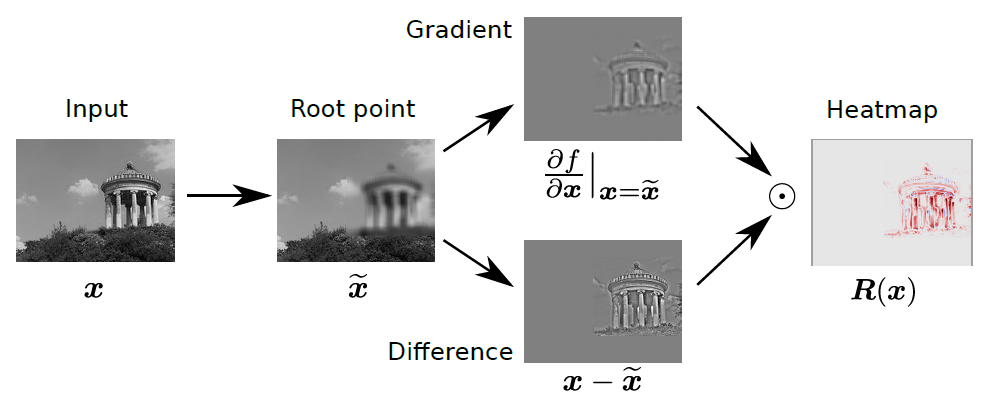
\includegraphics[width=0.5\textwidth]{images/fig._2_example_root_point}
	\caption{Example: Root point in an image.}
	\label{fig.2}
\end{figure}
Since an image possibly can have more than one root point the choice is crucial and a good root point deviates from the original point $x$ as few as possible, i.e. minimizing the obective:
\begin{align*}
    \min_{\xi} ||\xi-x||^2 \text{ subject to } f(\xi) \text{     and   }\xi \in \mathbb{X},
\end{align*}
where $\mathbb{X}$ is the input domain.\\
Next we focus on the deep taylor decomposition, where we consider the mapping of neurons in one layer to each neuron in the next layer, assuming a relation explainable by some relevance function $R_j(\{x_i\})$. If this assumption holds and we further can identify a root point $\{\tilde{x_i}\}$ such that $R_j(\{\tilde{x_i}\}=0$ we can write equation \ref{eq:taylorDecomp}:
\begin{align*}
    \sum_j R_j= \left( \frac{\partial (\sum_j R_j)}{\partial \{x_i\}}\big|_{\{\tilde{x_i}\}}\right)^T \cdot (\{x_i\}-\{\tilde{x}\}) + \epsilon
    = \sum_i \sum_j \frac{\partial R_j}{\partial x_i}\big|_{\{\tilde{x}\}} \cdot (x_i-\tilde{x_i}) + \epsilon
\end{align*}
If definition \ref{thm:consistent} holds, the relevances is guaranteed to be conserved in each layer, i.e. $R_f=...=\sum_j R_j=...=\sum_p R_p$ and $R_f,...,\{R_j\},...\{R_p\} \geq 0$.\\
Further I will present two different approaches, the $\omega^2$-rule and the $z$-rule.\\
As a starting point we consider a simple detection pooling neural network with a reluctified linear activation function, i.e.
\begin{align*}
x_j = \max(0, \sum_i x_iw_{i,j} + b_j),\ x_k = \sum_j x_j,
\end{align*}
where $\{x_i\}$ is a d-dimensional input and $\theta = \{w_{i,j},b_j\}$ are weights and bias. To guarantee the exististence of a root point in the origin $b_j\leq0$. The relevance of the top layer is due to the pooling $R_k=\sum_j x_j$ and can be redistributed to the next layer according to the taylor decomposition
\begin{align*}
R_j = \frac{\partial R_k}{\partial x_j}\Big|_{\{\tilde{x}_J\}} \cdot (x_j - \tilde{x}_j) 
\end{align*}
If either $\sum_j\tilde{x}_j=0$ and $\forall j: \tilde{x}_j \geq0$ we need to chose $\{\tilde{x}_j\}$ resulting in $R_j = x_j$, since $\frac{\partial R_k}{\partial x_j} = 1$. Redistributing the relevance to the next layer using the taylor decomposition leads to 
\begin{align}
R_j = \sum_j\frac{\partial R_j}{\partial x_i}\Big|_{\{\tilde{x}_i\}^{(j)}} \cdot (x_i - \tilde{x}_i^{(j)})
\label{equ:propagationRule}
\end{align}
which is the starting point for the further analysis.


\subsection{Unconstrained Input Space and $\omega^2$-Rule}
\label{sec:wRule}
If we consider an unconstrained input space one can chose the nearest root point in the Euclidean sense. Considering the reluctified linear activation the intersection of the equation $\sum_i \tilde{x}_i^{(j)} w_{i,j}+b_j$ and the line of maximum descent defined by the derivative $\{\tilde{x}_i\}^{(j)}=\{x_i\} +tw_j$, where $w_i$ ist the weight vector and $t \in \mathbb{R}$. The root point is then given by $\{\tilde{x}_i\}^{(j)} = \{x_i - \frac{w_{ij}}{\sum_i w_{ij}^2}(\sum_i x_i w_{ij}+b_j)\}$ which leads by pluggin in \ref{equ:propagationRule}
\begin{align*}
R_i = \sum_j\frac{w_{ij}^2}{\sum_i w_{ij}^2} R_j
\end{align*}

\begin{proposition}[w-Rule consistency]
\label{prop:wconsistency}
$\forall g \in G$, the deep Taylor decomposition with the $w^2$-rule is consistent in the sense of Definition 3.
\end{proposition}

\subsection{Constrained Input Space and the z-Rules}
\label{sec:zRule}
Since in many cases the input domain is restricted the authors present a rule for bounded input spaces as well. Montavon et. al consider in their paper two possible spaces, first $\mathbb{X} = \mathbb{R}_x^d$ and $\mathbb{B} = \{\{x_i\} : \forall_{i=1}^d l_i\leq x_i \leq h_i\}$, where $l_i$ and $h_i$ are the respective lower and higher bounds for each input feature. I will only cover the first case since logic and results are quiet similar and the domain corresponds to the rectified linear activation. Hence we already know of the existence of one root at the origin we search on the segment $(\{x_i 1_{w_{ij}<0}\},\{x_i\})$ and thus the direction of the segment is given by $v_i^{(j)} = x_i - x_i 1_{w_{ij}<0} = x_i 1_{w_{ij}\geq0}$. If we follow the same logic is in section but change the line of maximum descent to $\{\tilde{x}_i\}^{(j)}=\{x_i\} +tx_i 1_{w_{ij}\geq0}$ we get the following relevance propagation rule
\begin{align*}
R_i = \sum_j\frac{x_i 1_{w_{ij}\geq0}}{\sum_{i´} x_{i´} 1_{w_{i´j}\geq0}} R_j
\end{align*}
\begin{proposition}[z-Rule consistency]\label{prop:zconsistency}
$\forall g \in G$, the deep Taylor decomposition with the z-rule is consistent in the sense of Definition 3.
\end{proposition}

\subsection{Deep Neural Networks}
Since many neural networks use complex deep architectures the authors further show a tractable way for the mapping of relevance from higher to the lower layers and introduce the concept of relevance models. The Min-Max and the Training-Free relevance model are introduced in the paper, however I will only cover the first. It is defined as 
\begin{align*}
y_j = \max(0, \sum_i x_i v_{ij} + a_j), \text{  } \hat{R}_k = \sum_j y_j,
\end{align*}
where $a_j = \min(0,\sum_lR_lv_{lj} + d_j)$ is a negative bias where the sum runs over the detection neurons from the upper layer and $R_l$ are the corresponding relevances. After estimation of the paramters $\{v_{ij}, v_{lj}, d_j\}$ by minimizing 
\begin{align}
min\langle(\hat{R}_k - R_k)^2\rangle 
\label{min:relevanceModel}
\end{align}
, where $R_k$ and $\hat{R}_k$ are the true and predicted relevances, we end up with the same problem as in section \ref{sec:main}. Due to the similar structure we can apply the same computations and compute $R_j = y_j$ and $R_i = \sum_j \frac{q_{ij}}{\sum_{i´}q_{i´j}} R_j$, where $q_{ij} = \{v_{ij}^2, x_iv_{ij}\}$ for the $w^2$-rule and z-rule, respectively. In contrast to the problem before the resulting heatmap is only approximately conservative, due to the possible errors during the minimization of  \ref{min:relevanceModel}. 



\section{Experiment}
\label{sec:exp}
As mentioned in the beginning the authors focus on image recognition and present examples from the MNIST and the ILSVRC data sets. I will only present one example from the MNIST data set and conclude with a self made example from the titanic data set.  

\subsection{MNIST Example}

\subsection{Titanic Example}


\section{Conclusion}
\label{sec:conclusions}
During the last years the importance of explainability of complex machine learning models became more and more present, due to either simple questions of understanding or even leag issues in for example pricing of insurances. Montavon et al. present in their paper \textit{Explaining NonLinear Classification Decisions with Deep Taylor Decompositions} practical algorithms which can help to tackle the problem of interpreteability for a wide range of deep learning models. the authors furthermore substantiate their theory with examples on two very famous image recognition data sets, namely the MNIST and the ILSVRC data sets. I myself could also reproduce very reliable results on the titanic data set which is in contrast to the other two a simple supervised binary classification problem.


\bibliographystyle{siamplain}
\bibliography{references}
\end{document}
